%%%%%%%%%%%%%%%%%%%%%%%%%%%%%%%%%%%%%%%%%
% a0poster Portrait Poster
% LaTeX Template
% Version 1.0 (22/06/13)
%
% The a0poster class was created by:
% Gerlinde Kettl and Matthias Weiser (tex@kettl.de)
% 
% This template has been downloaded from:
% http://www.LaTeXTemplates.com
%
% License:
% CC BY-NC-SA 3.0 (http://creativecommons.org/licenses/by-nc-sa/3.0/)
%
%%%%%%%%%%%%%%%%%%%%%%%%%%%%%%%%%%%%%%%%%

%----------------------------------------------------------------------------------------
%	PACKAGES AND OTHER DOCUMENT CONFIGURATIONS
%----------------------------------------------------------------------------------------

\documentclass[a0,portrait]{a0poster}

\usepackage{multicol} % This is so we can have multiple columns of text side-by-side
\columnsep=75pt % This is the amount of white space between the columns in the poster
\columnseprule=1pt % This is the thickness of the black line between the columns in the poster

\usepackage[svgnames]{xcolor} % Specify colors by their 'svgnames', for a full list of all colors available see here: http://www.latextemplates.com/svgnames-colors

%\usepackage{times} % Use the times font
\usepackage{palatino} % Uncomment to use the Palatino font

\usepackage[ngerman]{babel}
\usepackage[utf8]{inputenc}
\usepackage[german=quotes]{csquotes}


\usepackage{graphicx} % Required for including images
\graphicspath{{figures/}} % Location of the graphics files
\usepackage{subcaption} 
\usepackage{float}
\usepackage{booktabs} % Top and bottom rules for table
\usepackage[font=small,labelfont=bf]{caption} % Required for specifying captions to tables and figures
\usepackage{amsfonts, amsmath, amsthm, amssymb} % For math fonts, symbols and environments
\usepackage{wrapfig} % Allows wrapping text around tables and figures
\usepackage[export]{adjustbox}

\usepackage[backend=bibtex]{biblatex}
\bibliography{references} 
\renewcommand*{\bibfont}{\footnotesize}

\begin{document}

%----------------------------------------------------------------------------------------
%	POSTER HEADER 
%----------------------------------------------------------------------------------------

% The header is divided into two boxes:
% The first is 75% wide and houses the title, subtitle, names, university/organization and contact information
% The second is 25% wide and houses a logo for your university/organization or a photo of you
% The widths of these boxes can be easily edited to accommodate your content as you see fit

\begin{minipage}[b]{0.75\linewidth}
\veryHuge \color{NavyBlue} \textbf{Die MultiLA Softwareplattform} \color{Black}\\ % Title
\Huge\textit{Authoring Software und Learning Analytics für interaktive \mbox{Lernanwendungen} im Bereich Statistik und Data Science}\\[2cm] % Subtitle
\huge Markus Konrad MSc.\textsuperscript{1,2},
Prof. Dr. Maria Osipenko\textsuperscript{2},
Prof. Dr. Martin Spott\textsuperscript{1},
Prof.~Dr.~Andre Beinrucker\textsuperscript{1}\\[0.5cm] % Author(s)
\large \textsuperscript{1}Hochschule für Technik und Wirtschaft Berlin, \textsuperscript{2}Hochschule für Wirtschaft und Recht Berlin\\[0.4cm] % University/organization
%\Large \texttt{john@LaTeXTemplates.com} --- 1 (000) 111 1111\\
\end{minipage}
%
\begin{minipage}[b]{0.25\linewidth}

\includegraphics[width=15cm,right]{qrcode.png}
\captionof*{figure}{~~~~~~~~~~~~~~~~~~~https://ifafmultila.github.io/}
\end{minipage}

\vspace{1cm} % A bit of extra whitespace between the header and poster content

%----------------------------------------------------------------------------------------

\begin{multicols}{2} % This is how many columns your poster will be broken into, a portrait poster is generally split into 2 columns

%----------------------------------------------------------------------------------------
%	ABSTRACT
%----------------------------------------------------------------------------------------

%\color{Navy} % Navy color for the abstract
%
%\begin{abstract}
%
%Interaktive Lernanwendungen erweisen sich als nützliche Ergänzung zu Lehrmaterialien speziell in Statistik und Data Science, da sie ermöglichen, mathematische Theorie, interaktive Visualisierungen, Programmierübungen und andere Aufgaben in einer einzigen Umgebung zu kombinieren. In diesem Artikel stellen wir unsere Softwareplattform MultiLA vor, das ein Autorentool zur Erstellung von Lernanwendungen und ein Backend zur Datenerfassung umfasst. Die Software ermöglicht es, das Verhalten der Lernenden von Mausklicks und Mauszeigerbewegungen bis hin zum Erfolg beim Abschluss von Übungen nachzuverfolgen. Mit Hilfe von Learning Analytics können Lernverhalten und Lernerfolg analysiert werden, um die Anwendungen zu verbessern und die Lernenden zu unterstützen.
%
%\end{abstract}


%\color{DarkSlateGray} % DarkSlateGray color for the rest of the content
\color{black}

\section*{Einleitung}

Mittels der \textit{MultiLA Softwareplattform} ist es möglich, webbasierte, interaktive Lernanwendungen (im folgenden nur kurz als \enquote{Apps} bezeichnet) zu entwickeln, diese den Studierenden zur Verfügung zu stellen und auf datenschutzkonforme weise Interaktionsdaten der Studierenden mit den Apps zu sammeln, sowie Experimente durchzuführen. Damit werden drei Ziele erreicht:

\begin{itemize}
    \item Verbesserung der Lehre durch innovative, interaktive Lernanwendungen,
    \item Unterstützung der Forschung im Bereich Learning Analytics,
    \item Verbesserung der Apps durch den aus den Daten gewonnenen Erkenntnissen.
\end{itemize}

Die Softwareplattform wurde im Rahmen des IFAF MultiLA-Projekts an der HTW Berlin und der HWR Berlin entwickelt und steht komplett als Open Source Softwarepaket zur Verfügung. Das Projekt wurde bereits im Rahmen der \textit{UseR! Conference 2024} \cite{userconf24} vorgestellt. Ein wissenschaftlicher Artikel befindet sich gerade im Einreichungsprozess.

\subsection*{Hauptfeatures}

\begin{itemize}
    \item Erstellung interaktiver Apps mittels \textit{RMarkdown} oder als \textit{Shiny}-Anwendungen
    \item Hoch granulare, konfigurierbare und anonyme Nachverfolgung von Benutzerinteraktionen mit den Apps: Mausbewegungen, Klicks, Einreichen von Übungen usw.
    \item Unterstützung von A/B-Testexperimenten und integrierten Umfragen
    \item Konfigurierbare Apps erlauben mehrere Varianten einer einzigen Basisanwendung
%    \item Dynamische Zusammenfassungsleiste für Apps
    \item Webbasierte Administrationsoberfläche zum Veröffentlichen von Apps, Einrichten von Varianten und Experimenten sowie Herunterladen gesammelter Daten
%    \item Datenaufbereitungs- und Analyseskripte
    \item Datenschutzkonforme, selbst gehostete open-source Lösung
\end{itemize}

\section*{Von der Lernanwendung zu Learning Analytics}

\subsection*{1. Lernanwendungen erstellen}

Der inhaltliche Fokus liegt auf dem Bereich Statistik, Mathematik und Data Science. In diesem Bereich ist die Nutzung der Programmiersprache \textit{R} sowohl unter Lehrenden als auch in den Curricula sehr ausgeprägt, weshalb zur Erstellung der Apps \textit{RMarkdown} in Kombination mit \textit{RStudio} zum Einsatz kommen. Über einen Editor lassen sich Text, Formeln, Grafiken, Quizaufgaben und Code-Übungen einfügen. Komplexere interaktive Erklärelemente lassen sich mit \textit{Shiny} programmieren und direkt einbetten. Das von uns entwickelte R Paket \textit{learnrextra} \cite{konrad_ifafmultilalearnrextra_2024} enthält die Funktionen zum Aufzeichnen der Nutzungsdaten sowie Erweiterungen für mathematische Übungsaufgaben und das Einbetten von Umfragen.

\vspace{1cm}

\begin{figure}[H]
\hfill
\begin{subfigure}[h]{0.45\linewidth}
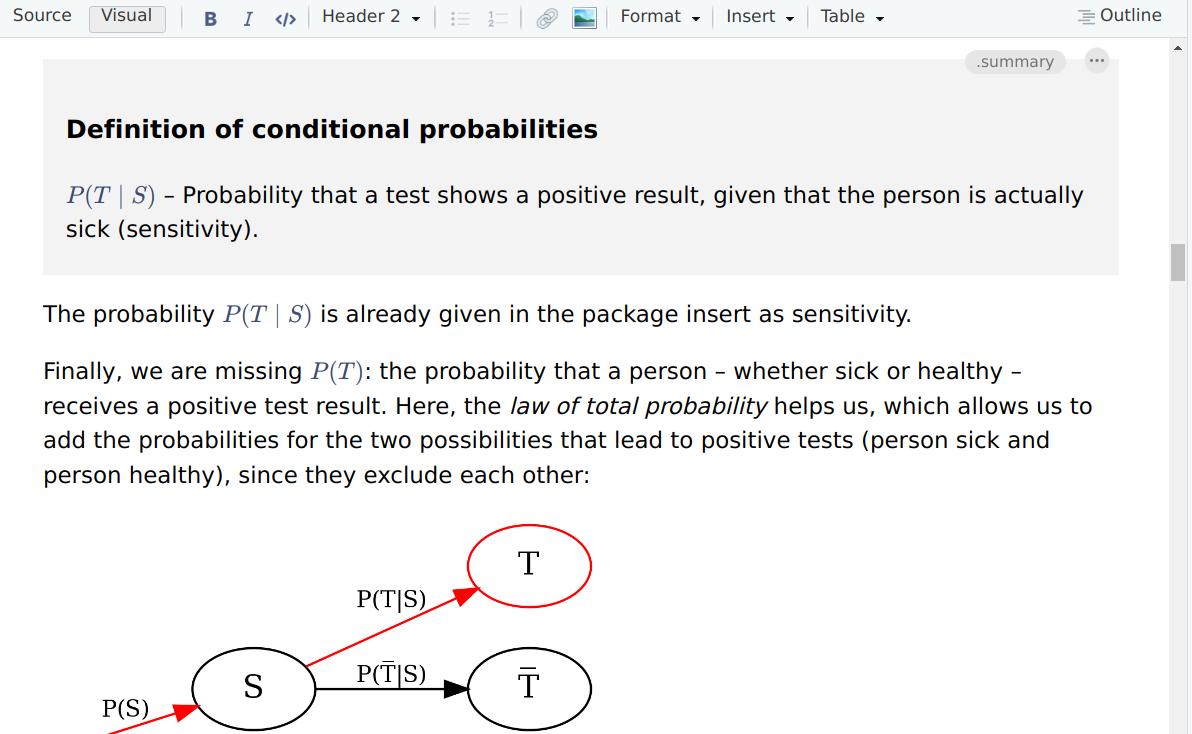
\includegraphics[width=\linewidth]{at-visual-smaller}
\caption*{\footnotesize Erstellen einer Lernanwendung in RStudio}
\end{subfigure}
\hfill
\begin{subfigure}[h]{0.45\linewidth}
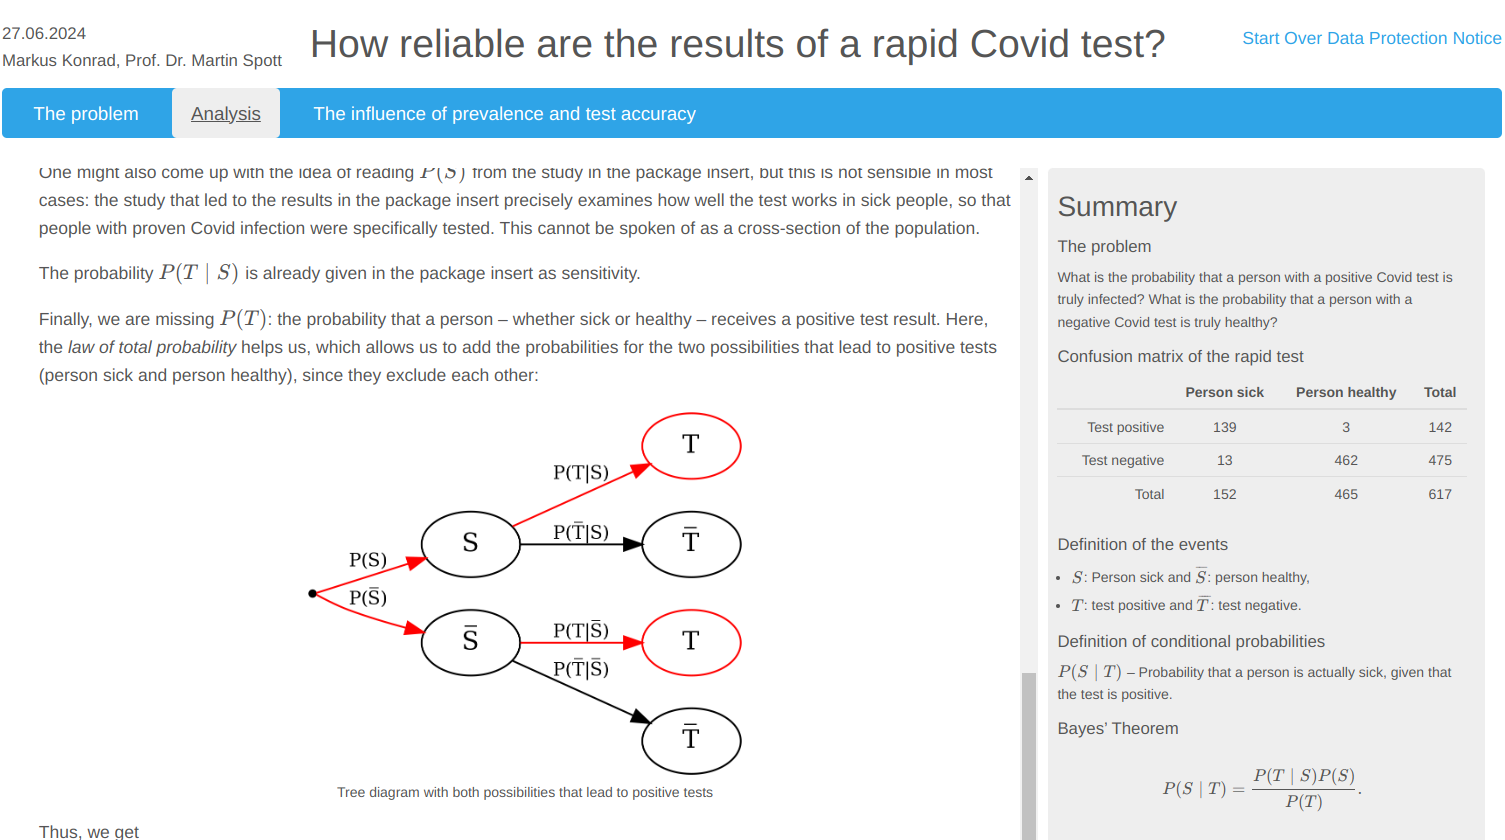
\includegraphics[width=\linewidth]{app-summary}
\caption*{\footnotesize Fertige App mit dynamischer Zusammenfassungsleiste auf der rechten Seite}
\end{subfigure}
\hfill
\end{figure}

\subsection*{2. Lernanwendungen bereitstellen}

Die entwickelte App kann im Anschluss auf einem Server bereitgestellt werden. Über den Administrationsbereich können verschiedene Varianten der selben App mittels Konfigurationen bereitgestellt werden. Zudem können Experimente in Form von A/B-Tests erstellt werden, um mehrere Apps oder Varianten mittels Zufallszuordnung zu den Studierenden miteinander zu vergleichen. Zur Datenminimierung lässt sich exakt einstellen, welche Art von Daten während der Nutzung der Apps gesammelt werden. Es wird schließlich ein Link erzeugt, den Lehrende an ihre Studierenden verteilen können.

Eine Datenaufzeichnung erfolgt nur nach Zustimmung und komplett anonym. Dabei wird beim ersten Besuch der App genau über die Umfang und den Zweck der erhobenen Daten informiert. Die Lernanwendung lässt sich selbstverständlich auch ohne Zustimmung zur Datenaufzeichnung verwenden.


\subsection*{3. Nutzungsdaten sammeln und auswerten}

Die Nutzungsdaten werden im Backend auf dem Server gespeichert und können auch über den geschützten Administrationsbereich heruntergeladen werden. Für die Verarbeitung der komplexen und umfangreichen Daten (bspw. Mausbewegungspfade) stellen wir fertige Analyseskripte in R zur Verfügung.

%\begin{center}\vspace{1cm}
%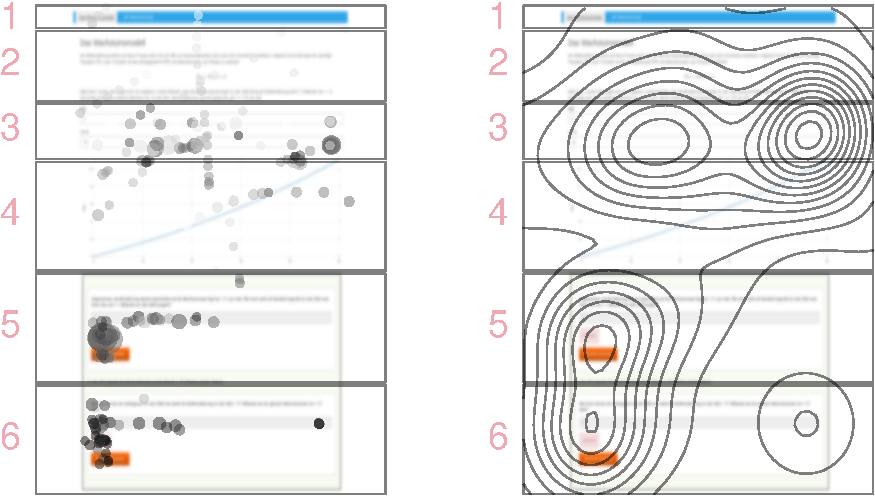
\includegraphics[width=0.5\linewidth]{figtraj-1}
%\captionof{figure}{Klicks und \enquote{Heatmap} einer App}
%\end{center}\vspace{1cm}


\begin{figure}[H]
\hfill
\begin{subfigure}[h]{0.6\linewidth}
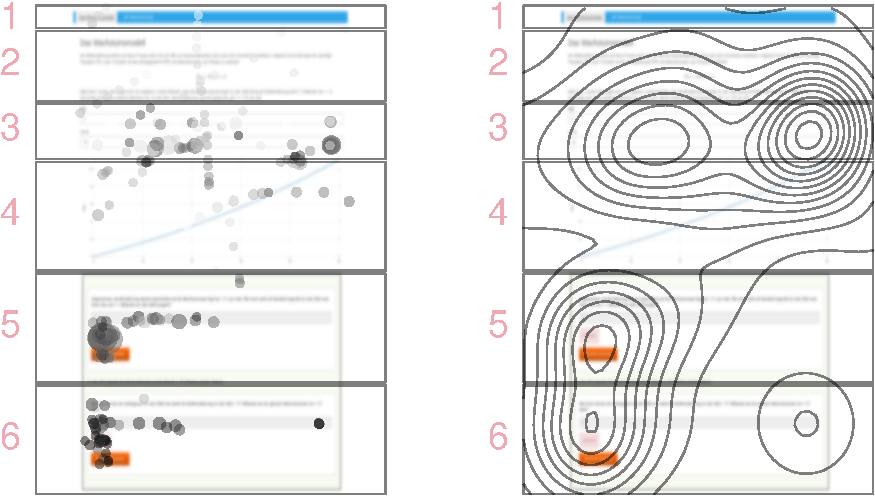
\includegraphics[width=\linewidth]{figtraj-1}
\caption*{\footnotesize \enquote{Heatmap} von Klicks in einer App}
\end{subfigure}
\hfill
\begin{subfigure}[h]{0.325\linewidth}
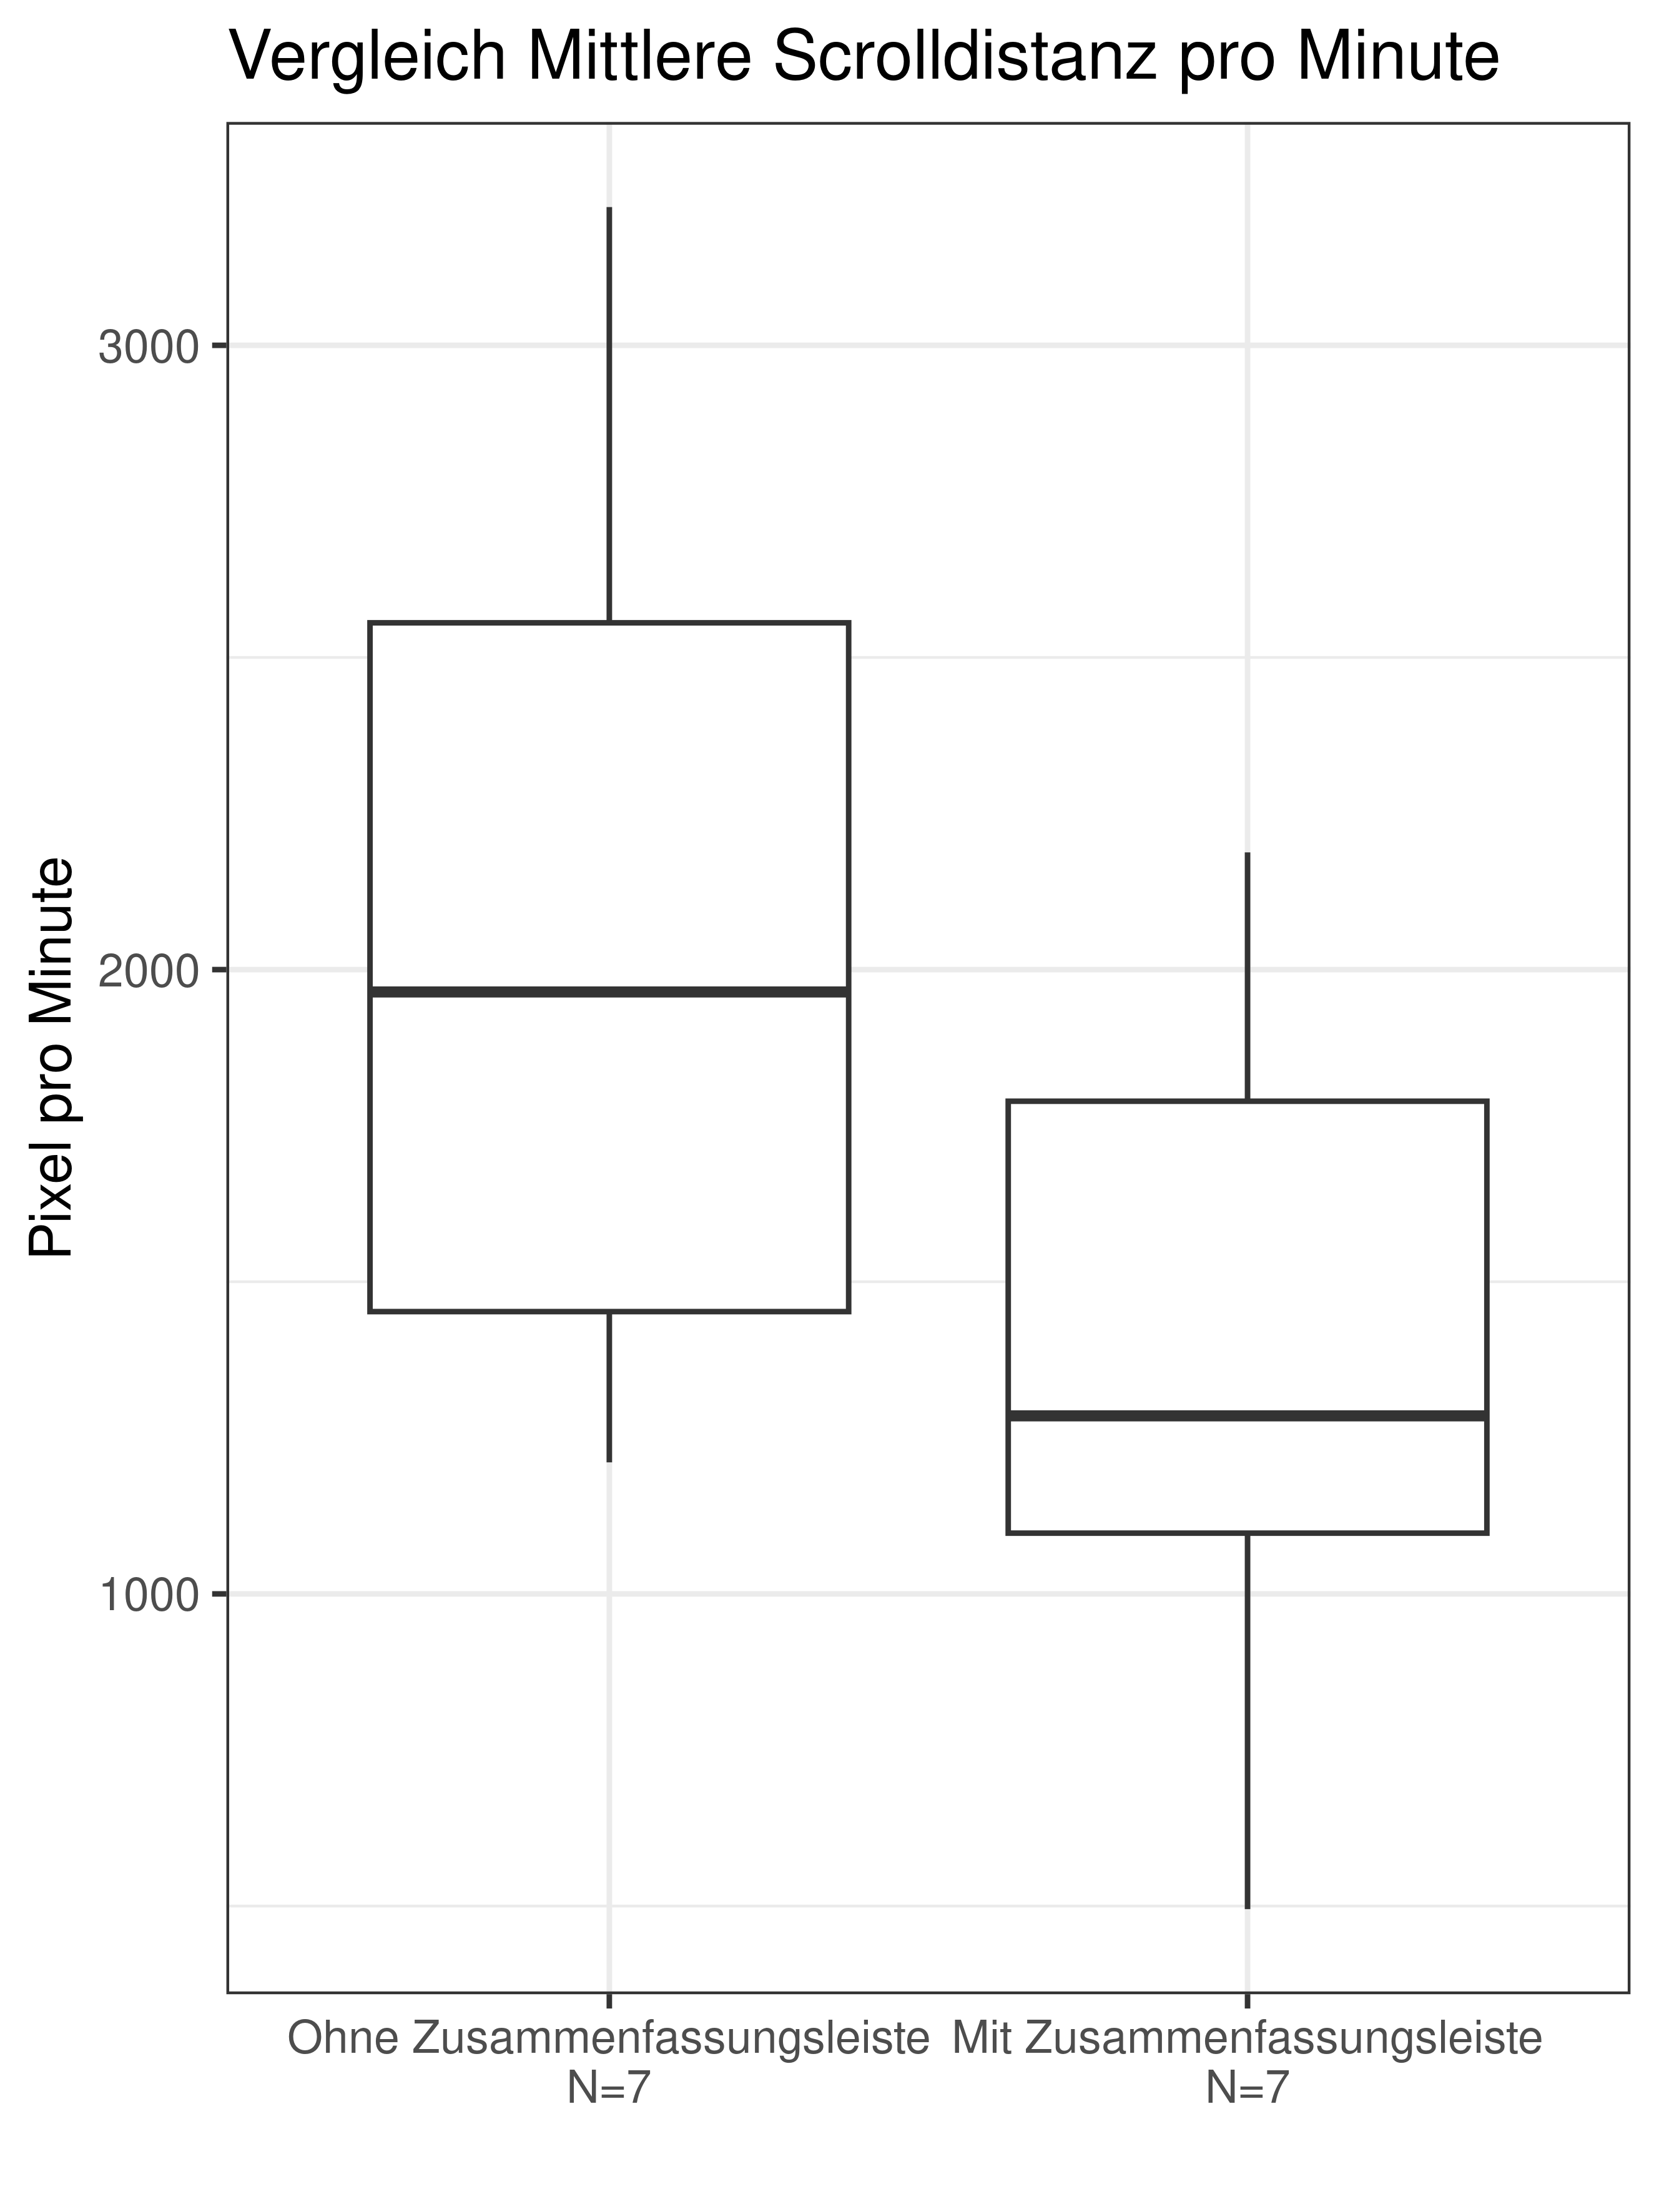
\includegraphics[width=\linewidth]{summarypanel_scrolldist_poster}
\caption*{\footnotesize Ergebnis eines A/B-Experiments: Ver\-änd\-erung des Scrollverhaltens durch die Zusammenfassungsleiste}
\end{subfigure}
\hfill
\end{figure}


%\begin{figure}[H]
%\hfill
%\begin{subfigure}[h]{0.45\linewidth}
%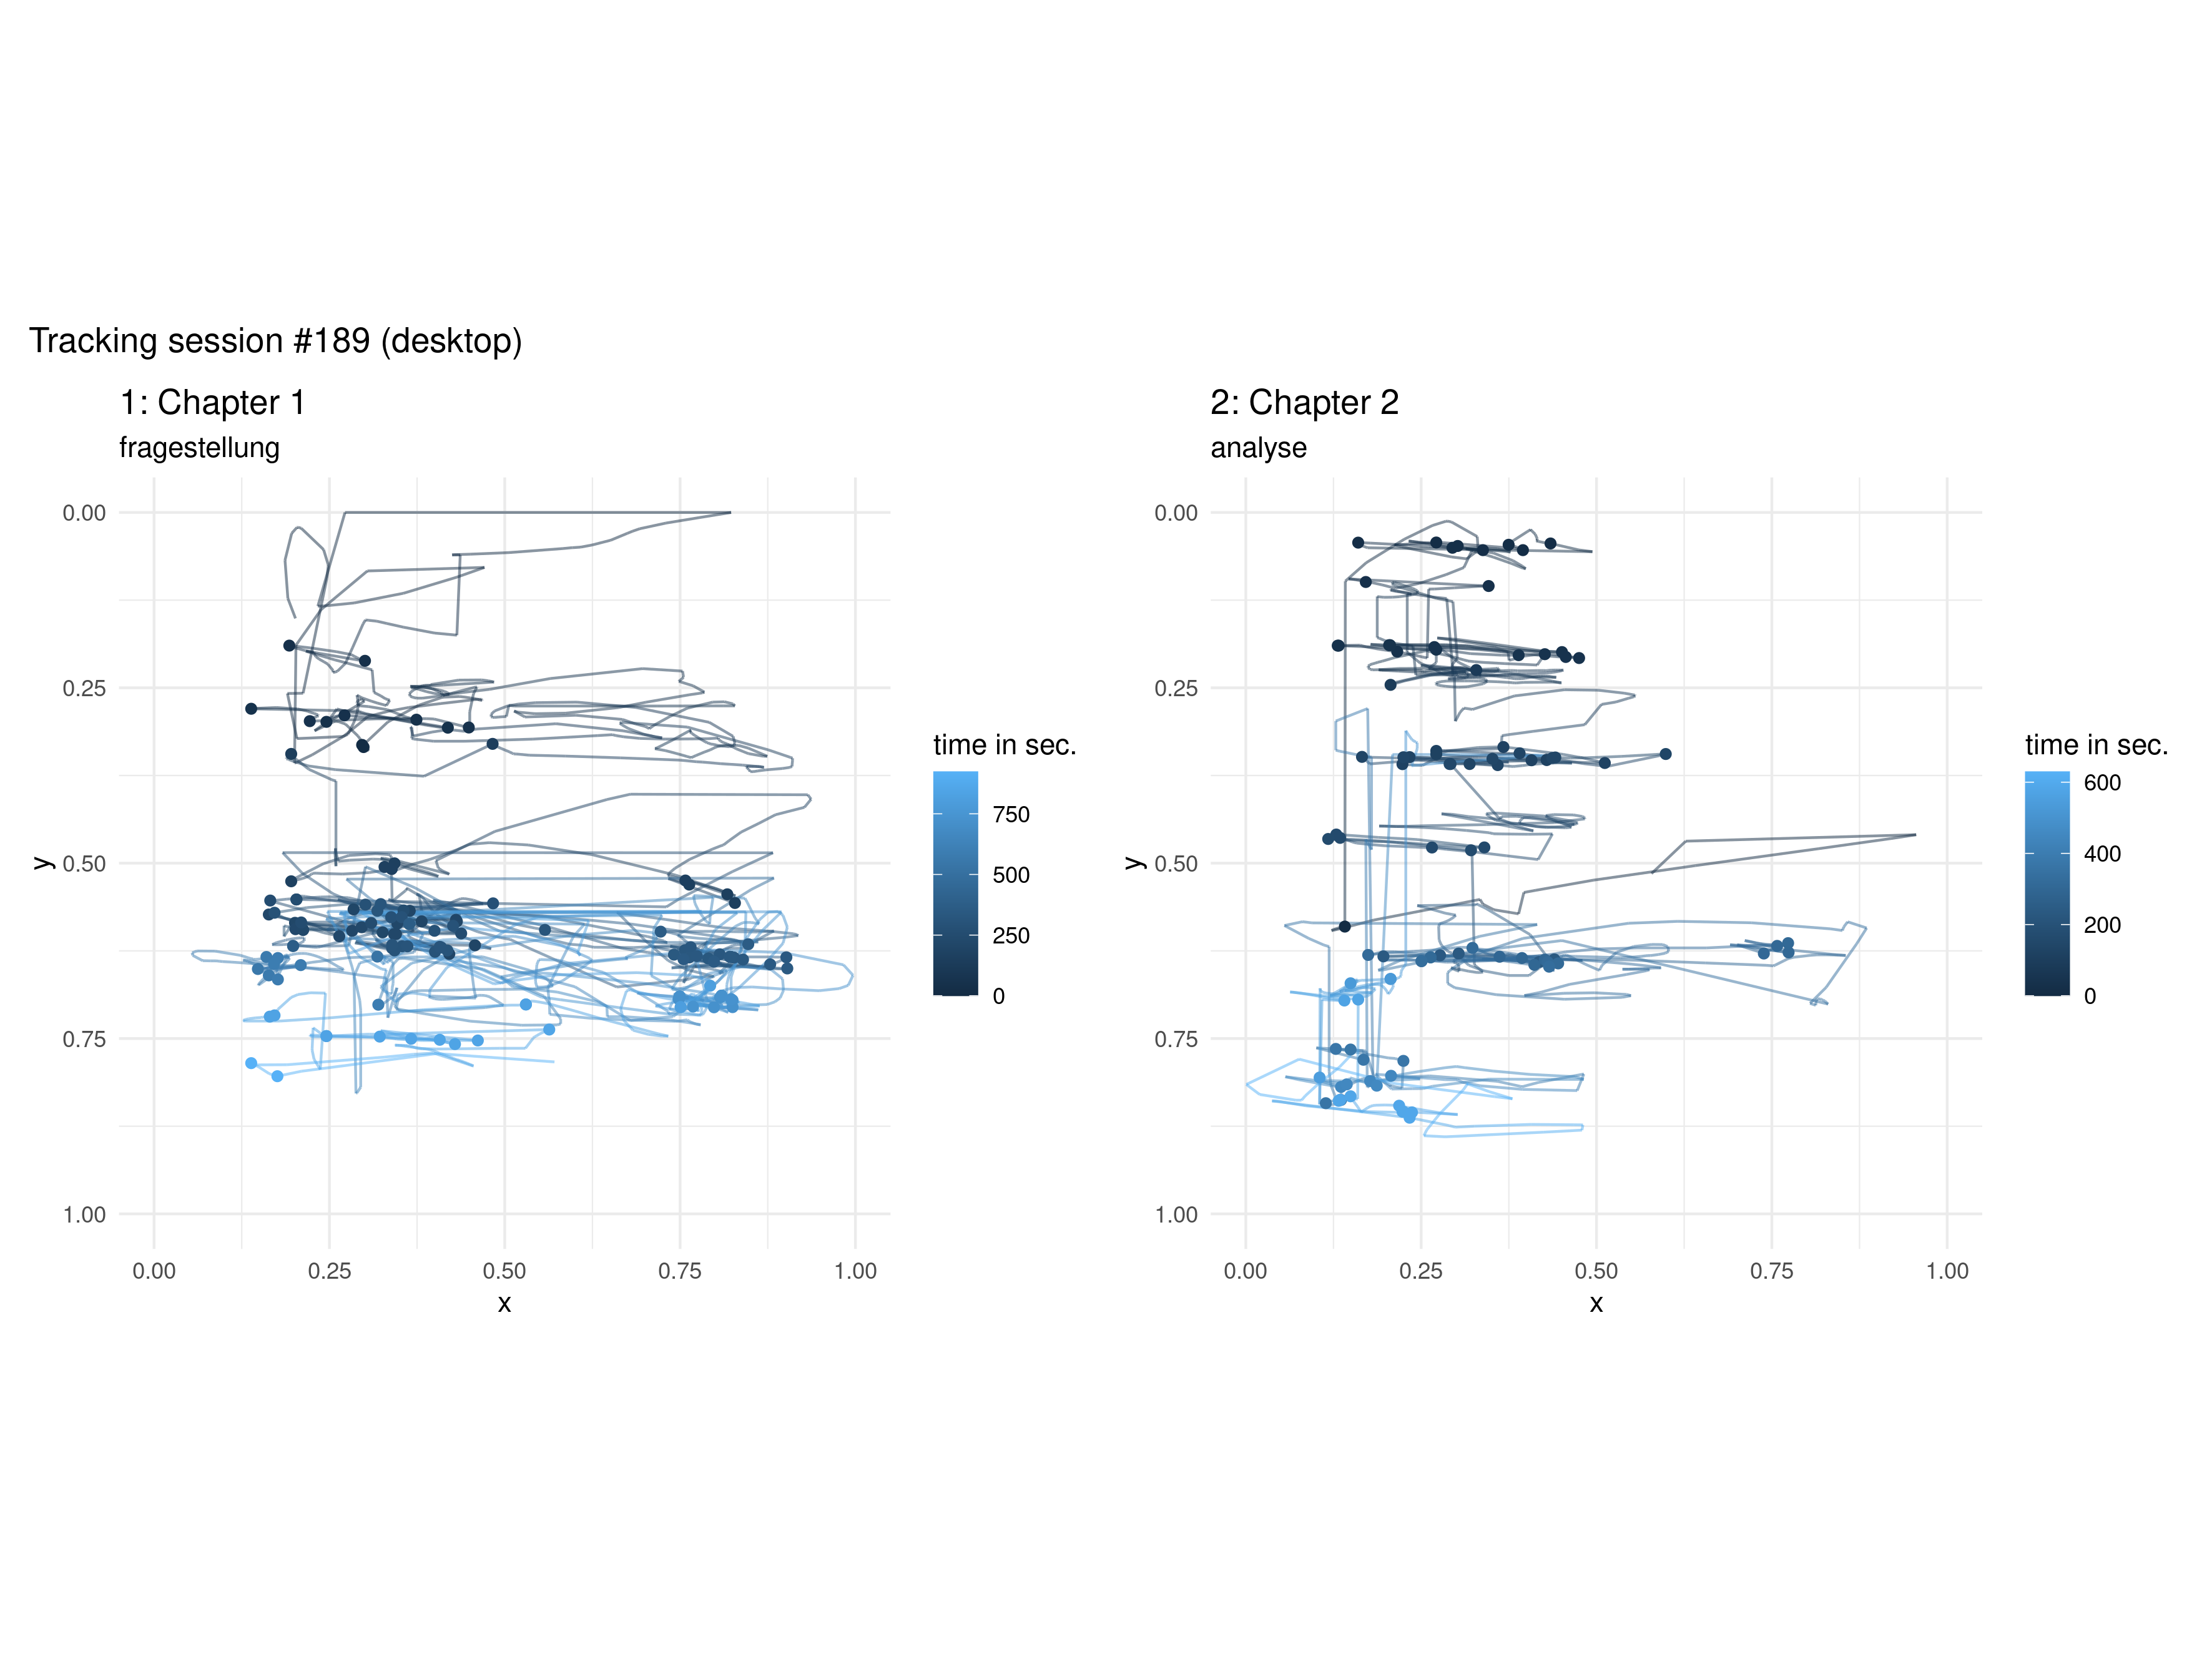
\includegraphics[width=\linewidth]{mouse_tracks_189}
%\caption{Mausbewegungen und Klicks in einer App}
%\end{subfigure}
%\hfill
%\begin{subfigure}[h]{0.45\linewidth}
%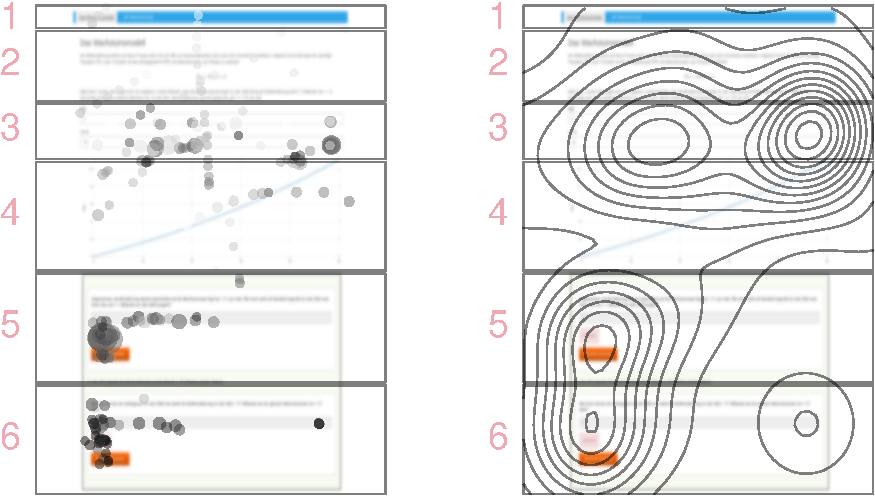
\includegraphics[width=\linewidth]{figtraj-1}
%\caption{\enquote{Heatmap} von Klicks in einer App}
%\end{subfigure}
%\hfill
%\end{figure}


%\section*{Hintergrund}
%
%\subsection*{Softwarearchitektur}
%
%\begin{center}\vspace{1cm}
%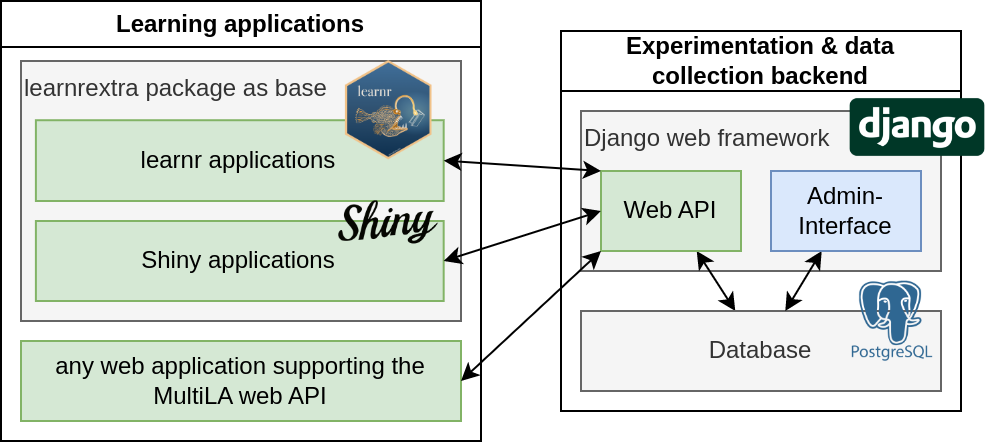
\includegraphics[width=0.6\linewidth]{sw-arch}
%\captionof{figure}{MultiLA Softwarearchitektur}
%\end{center}\vspace{1cm}

\section*{Erstellte Lernanwendungen}

Im Rahmen des Forschungsprojekts wurden zahlreiche interaktive Apps für die Lehre in Statistik und Data Science entwickelt. Die abgedeckten Themen umfassen u.a. Wahrscheinlichkeitstheorie, diskrete und stetige Wahrscheinlichkeitsverteilungen oder Benfords Gesetz.% Sämtliche Apps wurden bereits in der Lehre eingesetzt.

\begin{center}\vspace{1cm}
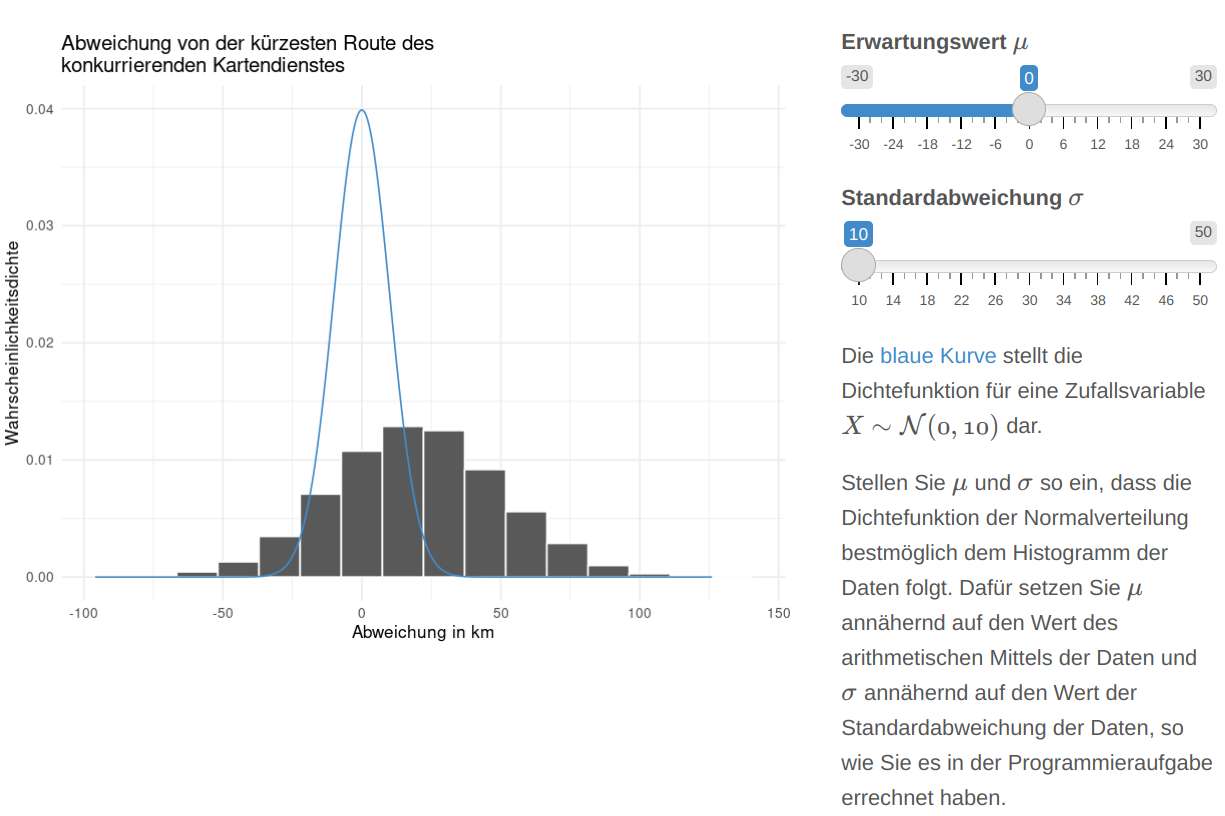
\includegraphics[width=0.6\linewidth]{wvstetig}
\captionof*{figure}{\footnotesize Beispiel einer Lernanwendung mit interaktiver Grafik}
\end{center}

%\vspace{1cm}
%\begin{figure}[H]
%\hfill
%\begin{subfigure}[h]{0.575\linewidth}
%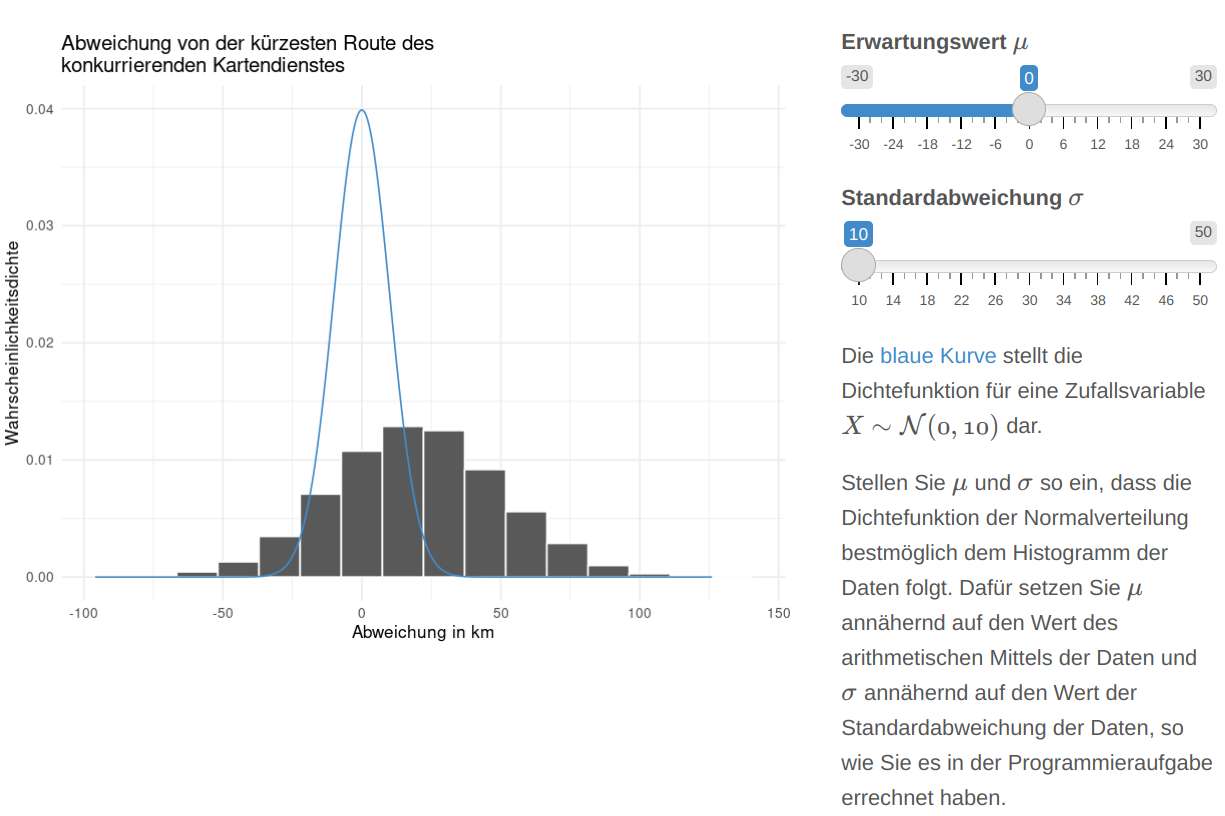
\includegraphics[width=\linewidth]{wvstetig}
%\caption{Beispiel einer Lernanwendung mit interaktiver Grafik}
%\end{subfigure}
%\hfill
%\begin{subfigure}[h]{0.325\linewidth}
%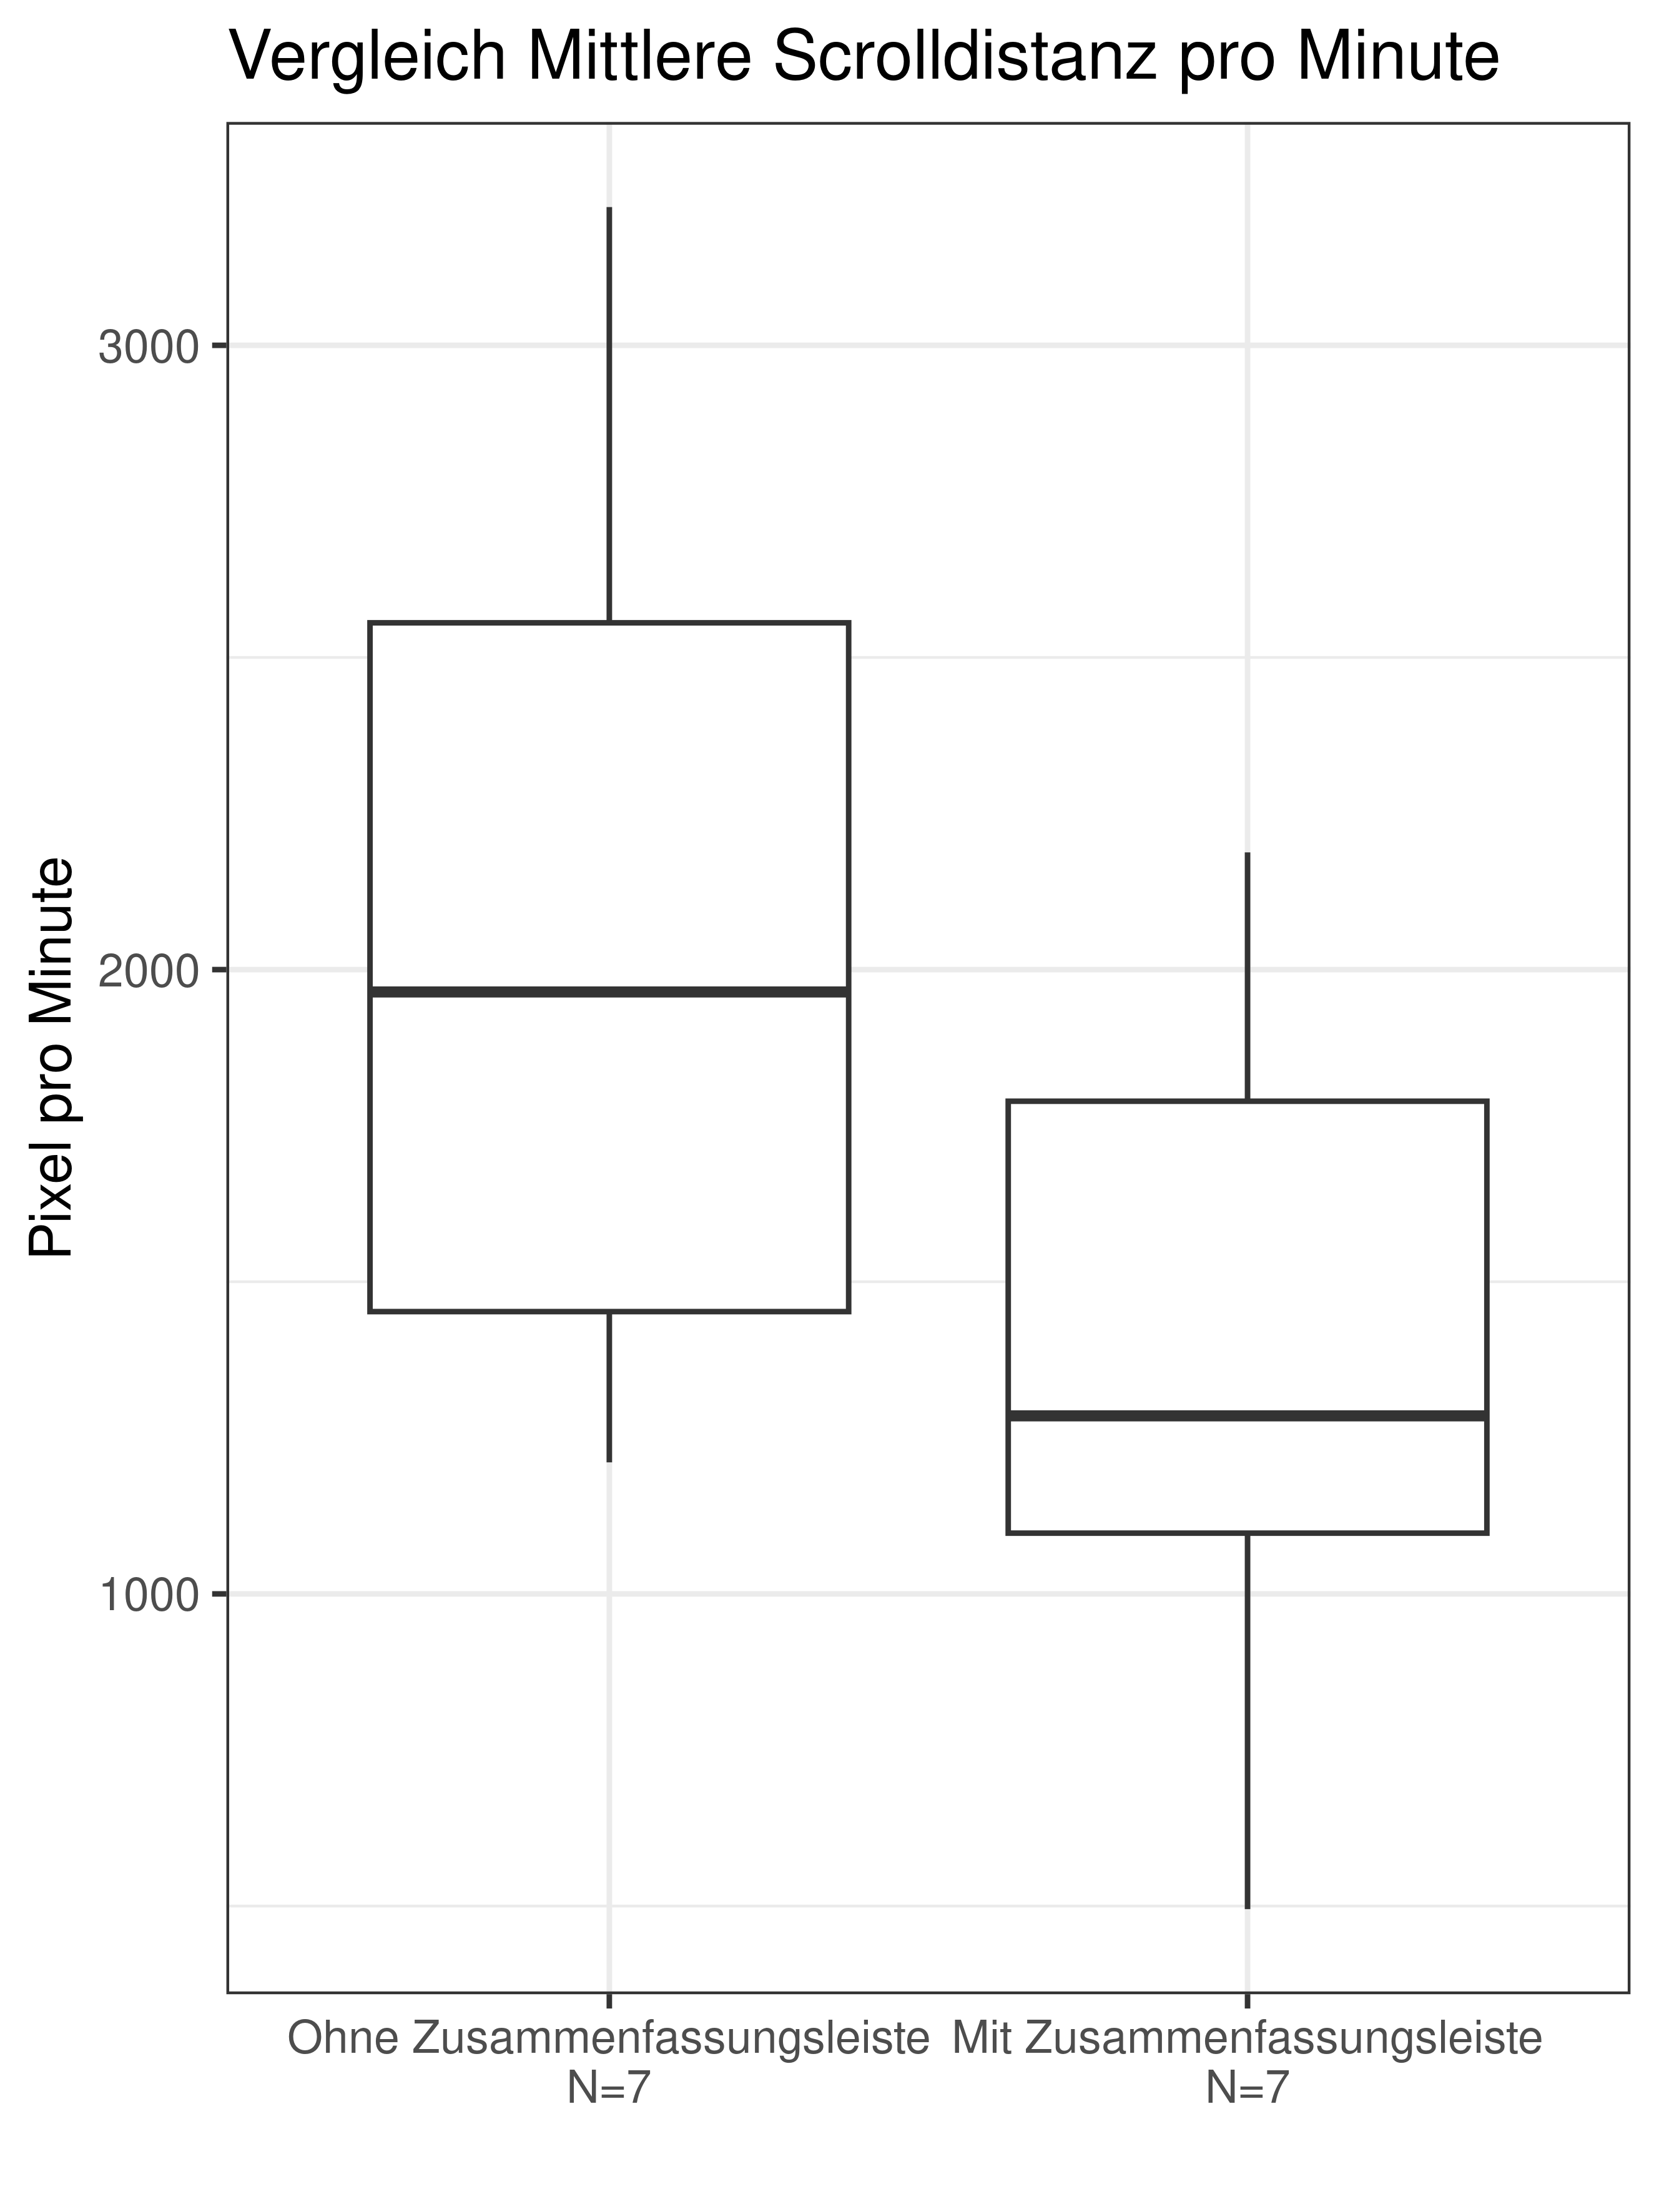
\includegraphics[width=\linewidth]{summarypanel_scrolldist_poster}
%\caption{Ergebnis eines A/B-Experiments: Weniger Scrollen durch Zusammenfassungsleiste}
%\end{subfigure}
%\hfill
%\end{figure}


\section*{Erste Auswertungen}

In den vergangenen zwei Semestern wurden die Apps in der Lehre eingesetzt, Daten gesammelt und anhand der daraus gewonnen Erkenntnisse die Apps kontinuierlich verbessert. Beispielsweise konnten wir durch die Einführung der dynamischen Zusammenfassungsleiste erreichen, dass Studierende weniger Zeit beim Heraussuchen wichtiger Informationen für das Lösen von Übungsaufgaben verbringen. Das konnten wir anhand eines A/B-Experiments mit unserer Softwareplattform und der Auswertung von Scrolldaten nachweisen. Zudem konnten wir durch die gewonnenen Daten ermitteln, bei welchen Aufgaben Verständnisprobleme vorherrschen und diese entsprechend anpassen. Eingebettete Umfragen erlauben uns jedes Semester die Zufriedenheit mit den angebotenen Apps abzufragen. Dabei stellte sich u.a. heraus, dass Studierende die interaktiven Apps überwiegend positiv aufnehmen und sowohl in den Laborübungen, als auch zu Hause stärker nutzen wollen.

\section*{Fazit und Ausblick}

Der gewählte Ansatz hat sich als äußerst flexibel erwiesen und hebt sich damit von bestehenden Lösungen für interaktive Lernanwendungen und Datensammlungs-Tools für Learning Analytics ab. Die Software ist frei verfügbar und kann damit datenschutzkonform auf Servern im eigenen Netz betrieben werden.

Einschränkend muss erwähnt werden, dass unsere Datenauswertungen bisher nur durch eine geringe Anzahl von Nutzungssessions gestützt werden. In den kommenden Semestern sollen kontinuierlich weitere Daten erhoben werden um die Auswertungen belastbarer zu machen, die Apps weiter zu verbessern und die MultiLA Softwareplattform damit weiteren Nutzungstests zu unterziehen. Des weiteren setzt das Bereitstellen von Apps  Kenntnisse in Serveradministration voraus – eine Hürde, die wir in Zukunft beseitigen wollen.

%----------------------------------------------------------------------------------------
%	REFERENCES
%----------------------------------------------------------------------------------------


\vspace{1cm}
\hrulefill
\vspace{1cm}
\printbibliography[heading=none]


\end{multicols}

%----------------------------------------------------------------------------------------
%	FOOTER
%----------------------------------------------------------------------------------------


\vspace{3cm}

\begin{minipage}[b]{0.33\linewidth}

\includegraphics[width=10cm,left]{htw_logo.jpg}
\end{minipage}
\begin{minipage}[b]{0.34\linewidth}

\includegraphics[width=10cm,center]{ifaf_logo.jpg}
\end{minipage}
\begin{minipage}[b]{0.33\linewidth}

\includegraphics[width=15cm,right]{hwr_logo.png}
\end{minipage}

\end{document}